% file siminos/froehlich/slice/singul.tex
% $Author$ $Date$

% \section{Slice {\sset}}
%	\label{sec:singul}

If  two patterns are close, their group orbits will be nearly parallel,
$\braket{\groupTan(\ssp)}{\sliceTan{}} \neq 0$, and for a smooth flow the
slice will be transverse to all group orbits in an open
neighborhood of the {\template} \slicep. However, looking back at
\refeq{SL:CLEsliceRot} and \refeq{eq:so2reduced}, we see that globally the
\mslices\ always introduces singularities in the \reducedsp. Two hyperplanes are
associated with  any given {\template} \slicep; the slice \refeq{PCsectQ0},
and the hyperplane of points \sspSing\ such that
\beq
\braket{\groupTan(\sspSing)}{\sliceTan{}}
 =
\braket{\sspSing}{\Lg^2\slicep}
 =0
%\,.
\ee{sliceSingl}
(for simplicity, in this section we specialize to the  $\SOn{2}$ case).
We shall refer to the $(d\!-\!2)$\dmn\ intersection of the two as
the {\em \sset} $S$ in the \reducedsp, $\sspRSing \in S \subset \pSRed$.
\beq
\braket{\groupTan(\sspRSing)}{\sliceTan{}}
 =
\braket{\sspRSing}{\Lg^2\slicep}
 =0
\,.
\ee{sliceSingl}
Looking back at \refeq{SO2inflPoint}, we see that this the locus
of inflection points, a hyperplane through which the curvature changes
sign, and a local minimum turns into a local maximum.
Just as the slice itself, the {\em \sset} goes through the origin.
For example, for \cLe\
$\sspRSing = (x_1^*,x_2^*,y_1^*,y_2^*,z)$,
$\slicep = (x_1',x_2',y_1',y_2',z)$,
and the 3\dmn\ {\sset} $\sspRSing \in S$ in the \reducedsp\ is given by
\[
0 = {x_1^* x'_1+x_2^* x'_2+y_1^* y'_1+y_2^* y'_2}
\,.
\]
The {\sset} is purely an artifact of the choice of a
{\template}, and has nothing to do with the dynamics; the corresponding full
\statesp\ trajectory is smooth.

The singularity in \refeq{SL:CLEsliceRot} for the \mframes\ rotation
angle $\gSpace$ is only apparent, as we now show by computing it for a
full \statesp\ trajectory $\ssp(\tau)$ that passes through the {\sset}
\refeq{sliceSingl} at time $\sspRSing =\ssp(\tau^*)$, which we shall set
to  $\tau^*=0$. At that instant the moving frame phase $\gSpace$ is
undefined: the numerator $\braket{\sspRSing}{\sliceTan{}}$ in
\refeq{SL:CLEsliceRot} vanishes as $\sspRSing$ is in the slice and
satisfies the slice condition \refeq{PCsectQ0}, and the denominator
${\braket{\groupTan_{}(\sspRSing)}{\sliceTan{}}}$ vanishes by
\refeq{sliceSingl}. Consider, however, the trajectory near the
singularity in the linear approximation,
$\ssp(\tau)\simeq\sspRSing+\vel(\sspRSing)\, \tau$:
\beq
\braket{e^{\gSpace \cdot \Lg}(\sspRSing+\vel(\sspRSing) \tau ))}
       {\sliceTan{a}}
    = \braket{e^{\gSpace \cdot \Lg}\vel(\sspRSing)}{\sliceTan{a}} \, \tau
\,.
\ee{singSetVelo}
$\gSpace$ approaches $\gSpace^*$ such that $\braket{e^{\gSpace^* \cdot
\Lg}\vel(\sspRSing)}{\groupTan(\slicep)}= 0$ so $\gSpace$ approaches an
angle that rotates $\vel(\sspRSing)$ into the slice.
All we are saying is
	\ifboyscout
\PCedit{give peace a chance.}
	\else
that as the full \statesp\ trajectory is smooth, the moving frame phase
$\gSpace$ goes smoothly through $\gSpace^*$, and at $\sspRSing$ we can
compute it either by interpolation, or by rotation the velocity
$\vel(\sspRSing)$ into the slice rather than rotating the \statesp\ point
\ssp.
	\fi

However, {\sset} crossing has a dramatic effect within the \reducedsp\: if
$\ssp(\tau)$ is a smooth trajectory in full {\statesp}, then the
\reducedsp\ flow $\sspRed(\tau)$ jumps whenever it crosses the {\sset}
$\sspRSing$.

We compute the size of the jump, and describe the behavior of nearby
trajectories.

Which angle it approaches before and after the singularity depends on the
restrictions put on the moving frame, and the trajectory can jump from
one $\gSpace$ to another depending on this choice.

The only
effect passing through a singularity will have on the \reducedsp\
trajectory then is to cause it jump from one point on a group orbit to
another at the singularity, and the trajectory will be smooth otherwise.



Suppose that a \reducedsp\ trajectory passes through a singularity at
time $\tau=\tau^*$, which we shall set to  $\tau^*=0$. At that instant
the numerator ?? in vanishes as $??$ is in the slice and satisfies
\refeq{eq:slicecondition} , and the denominator ?? vanishes by ??.

At the
singular instant, the group tangent of a point $\sspRed=\LieEl^{-1} \ssp$
lies in the slice, $\braket{\groupTan(\sspRed)}{\sliceTan{}}$ is zero,
and neither the velocity $\dot{\gSpace}(\tau)$ along the group tangent
nor the velocity in the slice are defined.

Formally the angular velocity ?? is undefined at $\ssp(\tau^*)$


% 2010-12-20 previously {CLEsingpass}{CLEnearsing2}
 \begin{figure}
 \begin{center}
(a)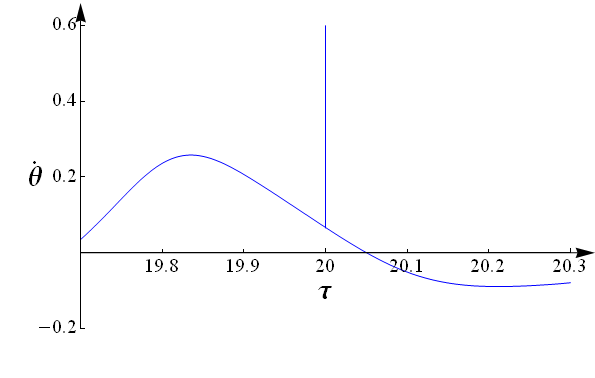
\includegraphics[width=0.45\textwidth]{dthetasing}%
(b)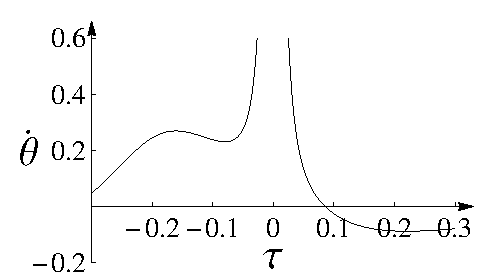
\includegraphics[width=0.45\textwidth]{dthetanearsing}%
 \end{center}
 \caption{\label{fig:dthetasing}
The {\groupVel} $\dot{\gSpace}$ for two \cLf\
\reducedsp\ trajectories in a slice defined by the
{\template} $\slicep$ given in \refeq{exmplTempl}:
 (a) As the trajectory $\sspRed(\tau)$ passes through the
singular point  $\sspRSing$ given in \refeq{exmplTempl},
the {\groupVel} diverges
$\dot{\gSpace} \to \infty$ as a Dirac delta function.
(b) The {\groupVel} for a nearby trajectory going
through $\sspRSing+\delta \sspRed$,
$\delta\sspRed=(0.01,0,0,0,0)$ exhibits a large
but finite excursion close to the singularity.
 }%
 \end{figure}

% 2010-12-20 previously {singpass}%
 \begin{figure}
 \begin{center}
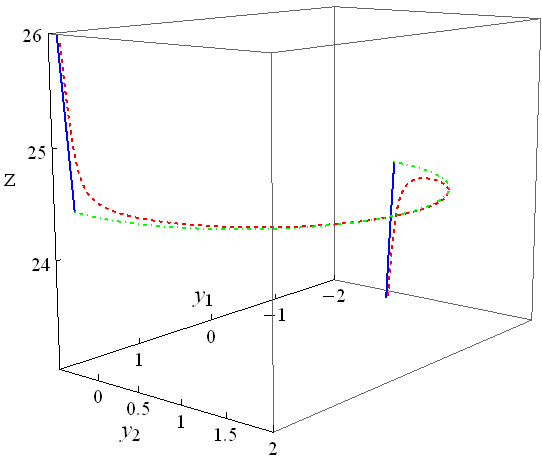
\includegraphics[width=0.45\textwidth]{singpass1}
 \end{center}
 \caption{\label{fig:singpass}
(color online).
Blow-up of a jump in \reffig{fig:Fullspace}\,(b), indicated by
a small rectangle.
(blue/dotted) A trajectory that passes through the singular point
$\sspRSing$ given in \refeq{exmplTempl}.
Note the instantaneous jump in the trajectory,  caused by the divergence in
velocity (\reffig{fig:dthetasing}\,(a)) as the trajectory
passes through the singularity. The red/dashed trajectory going
through $\sspRSing+\delta \sspRed$, $\delta \sspRed =(0,0,0.1,0,0)$,
makes a rapid transit around the singularity. The green trajectory is the group orbit of
$\sspRSing$ between the two $\gSpace$ that rotate $v(\sspRSing)$ in the
slice. Note also how the red/dashed trajectory begins near the
blue/dotted trajectory, closely follows the green trajectory after the
singularity point, reaches the other side of the blue/dotted arc and then
resumes closely following the blue/dotted trajectory.
 }%
 \end{figure}

To study this jump, consider a blow-up of the small rectangle indicated
in \reffig{fig:Fullspace}\,(b). For illustration purposes, the
	\PC{to SF - Please provide this secret numbers!}
{\template}
\bea
\slicep 	&=& (0.???,-0.???,-0.???,0.???,0)
	\continue
\sliceTan{} &=& (0.???,-0.???,-0.???,0.???,0)
	\label{exmplTempl} \\
\sspRSing	&=& (0.???,-0.???,-0.???,0.???,0)
\nnu
\eea
was determined by picking a point $\sspRSing = \ssp(0)$ from a segment of the
full \statesp\ ergodic trajectory $\ssp(\tau)$ and then computing \slicep\
such that $\sspRSing$ lies in the {\sset}.
As the trajectory $\sspRed(\tau)$ passes through the $\sspRSing$
the {\groupVel} diverges
$\dot{\gSpace} \to \infty$ as a Dirac delta function.
Nearby trajectories exhibit large excursions close to the singularity,
see \reffig{fig:dthetasing}.
    \PC{set $\tau = 0$ at the singularity in \reffig{fig:dthetasing}}


\reffig{fig:singpass}

In summary, the \reducedsp\ jumps in the flow induced by crossing the {\sset}
are harmless and theoretically under control, but numerically an unnecessary nuisance,
and preferably avoided by clever choices of slices.

%
% ****** End of file singul.tex ******
